\documentclass{article}
\usepackage{graphicx}
\usepackage{geometry}
\usepackage{amsmath}
\begin{document}

\section*{Problem statement}
I discretized the system dynamics as:
\begin{equation}
\begin{bmatrix}
\delta_{t+1} \\
\omega_{t+1} \\
\theta_{t+1}
\end{bmatrix}
=
\begin{bmatrix}
I & sI & 0 \\
sM^{-1}(K^I-B^{GG}) & I + sM^{-1}(K^P-D) & -B^{GL} \\
-{B^{LL}}^{-1}B^{LG} & {B^{LL}}^{-1}K^L_t & 0
\end{bmatrix}
\begin{bmatrix}
\delta_{t} \\
\omega_{t} \\
\theta_{t}
\end{bmatrix}
+
\begin{bmatrix}
0 \\
0 \\
{B^{LL}}^{-1}(P^L_t + \epsilon^L)
\end{bmatrix}
\label{eq:sysdyn}
\end{equation}
where $s$ is the step size, $t^*$ is the attack time, and
\begin{equation}
K^L_t =
\begin{cases}
0   & t < t^* \\
K^L & t \ge t^*
\end{cases}
\end{equation}
The goal is to find $t^*$ and $K^L$ given all other variables.
Measurements of the state variables $\delta$, $\omega$, and $\theta$ may be noisy;
all other variables are known exactly.
%Readings of the $P^L_t$ variable may be noisy, all other variables are known exactly.

\section*{Proposed Solution 1: Many Kalman Filters}

This is a naive baseline solution.

Let $K^L$ be an $m\times n$ matrix, and $\alpha$ be a hyperparameter.
For each $(i,j) \in \{1\dots m\}\times\{1\dots n\}$, let
${K^L}^{(i,j)}$ be the matrix with $\alpha$ in the $(i,j)$ position and $0$ everywhere else.
Let $MSE^{(i,j)}$ be the mean squared error of the Kalman filter's state estimate using ${K^L}^{(i,j)}$.
The idea is that $MSE^{(i,j)}$ will be close to zero when the attack occurs between nodes $i$ and $j$, and far away from zero everywhere else.

In practice, this method works well only when $\alpha$ happens to be very close to the true attack parameter.
Minor changes in $\alpha$, however, can cause large changes in the attack's profile,
resulting in a large mean squared error.

\section*{Proposed solution 2: Unscented Kalman Dual Estimation}

This is a slower, but slightly more robust solution.

Augment Equation \ref{eq:sysdyn} so that $K_t^L$ is one of the state variables.
This gives the (non-linear) system
\begin{equation}
\begin{bmatrix}
\delta_{t+1} \\
\omega_{t+1} \\
\theta_{t+1} \\
K^L_{t+1}
\end{bmatrix}
=
\begin{bmatrix}
I & sI & 0 & 0 \\
sM^{-1}(K^I-B^{GG}) & I + sM^{-1}(K^P-D) & -B^{GL} & 0\\
-{B^{LL}}^{-1}B^{LG} & {B^{LL}}^{-1}K^L_t & 0 & 0 \\
%-{B^{LL}}^{-1}B^{LG} & 0 & 0 & {B^{LL}}^{-1}\omega_t \\
0 & 0 & 0 & I
\end{bmatrix}
\begin{bmatrix}
\delta_{t} \\
\omega_{t} \\
\theta_{t} \\
K^L_t
\end{bmatrix}
+
\begin{bmatrix}
0 \\
0 \\
{B^{LL}}^{-1}(P^L_t + \epsilon^L) \\
0
\end{bmatrix}
\end{equation}
Now we can solve for $K^L_{t+1}$ using the unscented Kalman filter at the same time that we solve for the state variables.

%Solving the system directly results in slow convergence of the $K^L$ variable to the true value and a poor estimate of $t^*$.
Solving the system directly does not take advantage of $K^L$'s inherent sparsity.
A simple way to enforce sparsity is as follows:
after each update step for the UKF,
set $K^L_{t+1} = \text{softmax}(K^L_t)$.
The softmax ensures that only the most important components of the matrix are kept, but that we don't lose important information (e.g. the presence of multiple attacks, or an accidental mistake where the wrong component gets a high initial value).

\begin{figure}[T]
\includegraphics[width=0.3\textwidth]{example1-states}
\includegraphics[width=0.3\textwidth]{example1-K_L}
\includegraphics[width=0.3\textwidth]{example1-K_L-raw}
\caption{
    The results of method 2 on the example with 6 loads and 3 generators.
    The attack occurs at time 0.1.
    (left) The states.
    (center) The estimates of $K^L$ with softmax.
    (right) The estimates of $K^L$ without softmax.
}
\end{figure}

\begin{figure}[T]
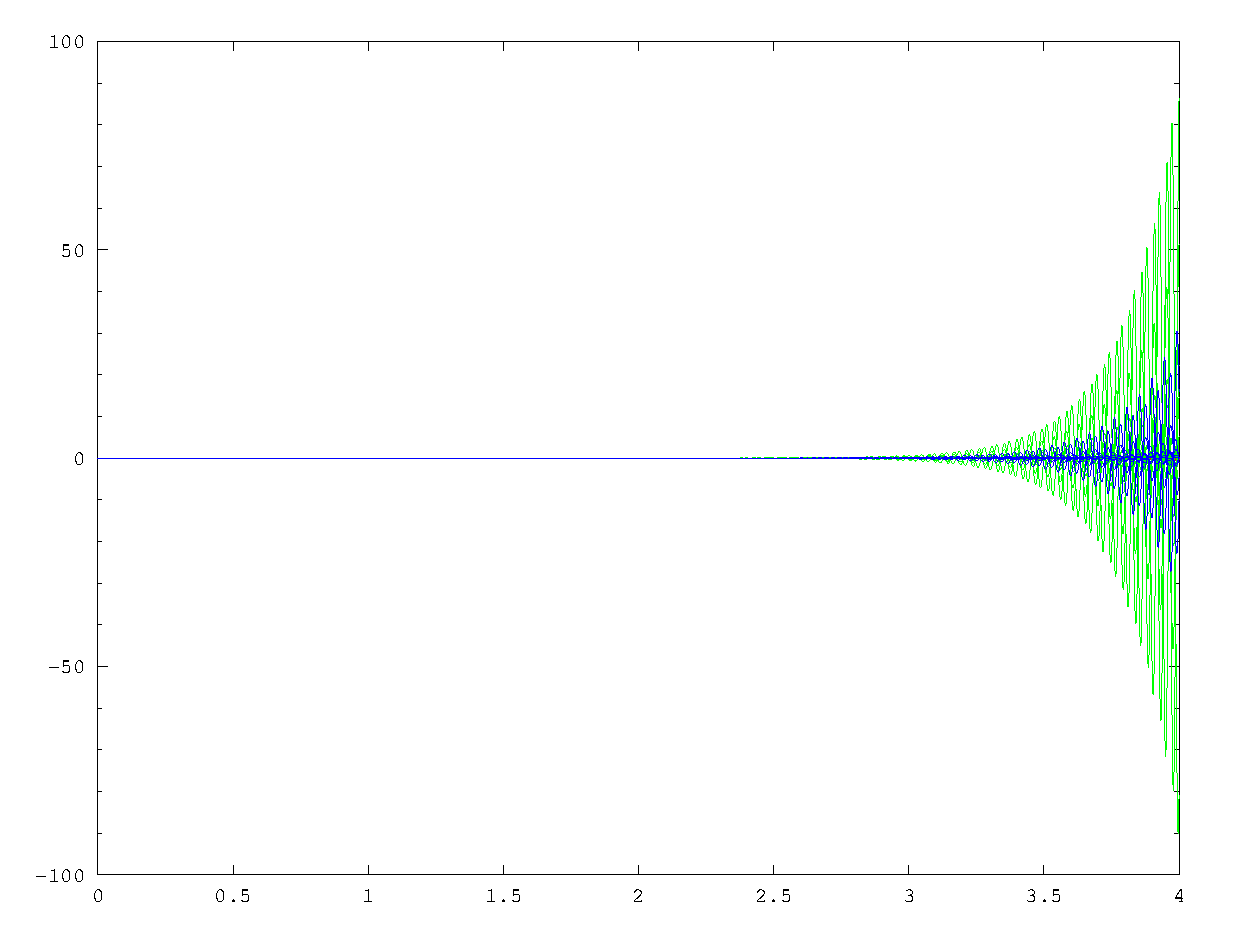
\includegraphics[width=0.3\textwidth]{random-8x10x25-states}
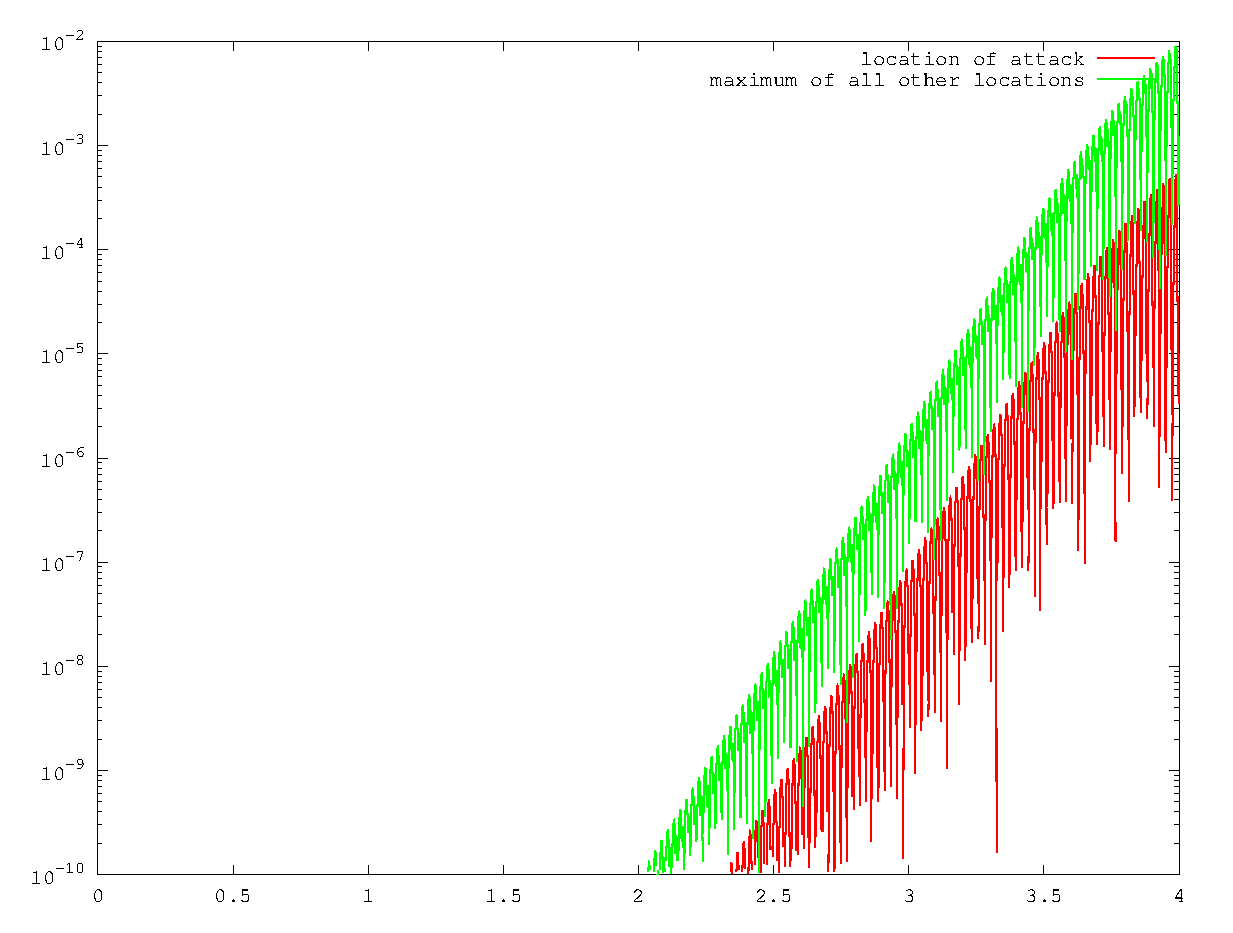
\includegraphics[width=0.3\textwidth]{random-8x10x25-K_L}
\includegraphics[width=0.3\textwidth]{random-8x10x25-K_L-raw}
\caption{
    The results of method 2 on a randomly generated power grid with 8 generators and 10 loads.
    The attack occurs at time 0.1.
    (left) The states.
    (center) The estimates of $K^L$ with softmax.
    (right) The estimates of $K^L$ without softmax.
    Without the softmax, we get a better estimate of $t^*$, but a poor estimate of $K^L$.
    With the softmax, the estimate of $t^*$ is delayed, but there is only a small number of non-zero entries in the estimated $K^L$ matrix.
}
\end{figure}

\end{document}
